\documentclass[aps,prd,reprint,nofootinbib,floatfix]{revtex4-2}

\usepackage{amsmath,amssymb,bm}
\usepackage{booktabs}
\usepackage{siunitx}
\usepackage{tikz}
\usepackage{xcolor}
\usepackage{hyperref}
\usepackage{microtype}
\linespread{1.025}
\setlength{\columnsep}{0.28in}
\usepackage{enumitem}
\usetikzlibrary{arrows.meta,calc,decorations.pathreplacing}

\hypersetup{
  colorlinks=true,
  linkcolor=blue!55!black,
  citecolor=blue!55!black,
  urlcolor=blue!55!black,
  pdftitle={A Helical Spacetime Ansatz Linking the Planck Scale and Electroweak Mixing},
  pdfauthor={Xiaodan Wu},
  pdfsubject={Helical spacetime geometry and a candidate geometric origin of the weak mixing angle},
  pdfkeywords={helical spacetime, emergent spacetime, weak mixing angle, Weinberg angle, Planck scale, quantum gravity, Emergent Frame}
}
\sisetup{separate-uncertainty=true}

\newcommand{\TEF}{\mathrm{TEF}}
\newcommand{\lp}{\ell_{\mathrm P}}
\newcommand{\hb}{\hbar}

\begin{document}

\title{A Helical Spacetime Ansatz Linking the Planck Scale and Electroweak Mixing}

% Author profile (kept consistent with arXiv/ORCID public identity)
\author{Xiaodan Wu}
\email{xiaodan@theemergentframe.org}
\affiliation{Independent Researcher}
\thanks{Research website: \href{https://theemergentframe.org}{theemergentframe.org}; ORCID: \href{https://orcid.org/0009-0005-5892-0293}{0009-0005-5892-0293}; DOI: \href{https://doi.org/10.5281/zenodo.22101000}{10.5281/zenodo.22101000}}

\date{August 20, 2026}

\begin{abstract}
We examine a minimal helical ansatz for microscopic spatial structure in which a primitive transverse radius is calibrated from the measured gravitational constant and the helix shape is subsequently fixed by a one-cycle phase-closure condition. The construction originates in the broader Emergent Frame (TEF) proposal, which treats spacetime as an emergent physical entity rather than a structureless pre-existing background, but the present paper is deliberately restricted to one concrete geometry and its quantitative consequence. Inspired mathematically by Euler's representation of planar rotation, a spatial line is modeled as a right-handed helix with radius $R$, axial advance per radian $a$, and dimensionless pitch ratio $q=a/R=\tan\beta$. A gravity--geometry calibration relation, using $G$ as an empirical input, gives $R_G=\sqrt{hG/(8\pi c^3)}=\ell_{\mathrm P}/2$. The model then distinguishes the axial extension generated in one turn from the helical arc length traversed internally: the former sets the cycle energy through the gravitational line-tension scale $c^4/G$, while the latter sets the cycle time. Requiring one complete primitive cycle to close its quantum phase, $E_{\rm cyc}T_{\rm cyc}/\hbar=2\pi$, yields $q\sqrt{1+q^2}=2/\pi$, so that $q\simeq0.556324$, $\beta_G\simeq29.088^\circ$, and $\sin^2\beta_G\simeq0.236348$. No electroweak observable enters this calculation. The resulting angle is therefore proposed only as a candidate primitive geometric reference for weak mixing, not as a completed derivation of the Weinberg angle. Its numerical proximity to the observed running weak-mixing parameter is presented as the reason this otherwise speculative spacetime ansatz merits further quantitative investigation.
\end{abstract}

\maketitle

\section{Introduction}

Microscopic spacetime models are not scarce, and geometric novelty by itself is not strong evidence for a new physical framework.  The motivation for the present paper is instead quantitative: a simple helical spacetime ansatz, once its dimensional scale is calibrated in the gravitational sector and its shape is fixed by an independent cycle condition, produces an intrinsic dimensionless angle that falls unexpectedly close to the electroweak weak-mixing parameter.  The logical direction is therefore from hypothesis to calculation to comparison, rather than from an electroweak target value back to a fitted geometry.

The geometric construction considered here originates in a broader emergent-spacetime proposal referred to as the Emergent Frame (TEF).  TEF treats spacetime not as a structureless, pre-existing arena but as a physical entity generated locally by matter.  The present paper does not attempt to establish the full framework.  It isolates one minimal assumption---that an elementary generated spatial line has a right-handed helical structure---and asks whether that assumption has a nontrivial quantitative consequence.

The standard descriptions of gravitation and electroweak physics begin from very different structures.  General relativity treats spacetime geometry as dynamical, whereas the electroweak sector is formulated as a gauge theory with group $SU(2)_L\times U(1)_Y$.  In the Standard Model the weak mixing angle is defined at tree level by
\begin{equation}
\tan\theta_W=\frac{g'}{g},
\label{eq:thetaW}
\end{equation}
where $g$ and $g'$ are the $SU(2)_L$ and $U(1)_Y$ gauge couplings, respectively \cite{PDG2026EW}.  Beyond tree level, numerical values associated with $\theta_W$ depend on the renormalization prescription and scale.

A mathematical inspiration for the helical representation is Euler's formula,
\begin{equation}
e^{i\phi}=\cos\phi+i\sin\phi.
\label{eq:euler}
\end{equation}
Euler's formula makes phase evolution and planar rotation two descriptions of the same mathematical structure.  It is not used here as evidence for the ansatz.  Rather, it suggests a compact representation in which the same parameter labels transverse rotation and longitudinal progression.  Writing the transverse coordinate as a complex variable,
\begin{equation}
w(\phi)=R e^{i\phi},\qquad z(\phi)=a\phi,
\label{eq:eulerhelix}
\end{equation}
produces the helical embedding used below.  The first expression is an Euler rotation in the transverse plane; the second is monotonic axial rollout.  Their combination gives a spatial line that advances while rotating.

There is a long history of attempts to interpret gauge structure and mixing geometrically, including Kaluza--Klein constructions and noncommutative geometry.  In the noncommutative-geometric program, the Standard Model coupled to gravity is encoded by a product of an ordinary spin manifold with a finite noncommutative geometry, leading to relations among gauge couplings at a unification scale \cite{Connes2006,ChamseddineConnesMarcolli2006}.  More recently, Monjo has investigated the weak mixing angle within a $U(1,3)$ colored-gravity construction and obtained interaction-dependent values of $\sin^2\theta_W$ from the generator structure of that model \cite{Monjo2025}.  A conceptually very different recent proposal by Liu, Low, and Yin selects a weak-mixing value close to experiment by minimizing quantum ``magic'' production in electroweak scattering \cite{LiuLowYin2025}.  These examples do not support the present ansatz directly; they instead illustrate that the empirical origin of the weak mixing angle continues to motivate attempts to derive it from structures deeper than the Standard-Model input couplings.

The idea that continuum spacetime itself may be emergent is likewise an active part of quantum-gravity research.  Contemporary examples range from spinor-based approaches to emergent Lorentzian geometry \cite{Rainer2026} to group-field-theory condensates in which continuum cosmological spacetime is reconstructed from collective quantum-geometric degrees of freedom \cite{CalcinariDelhomOriti2026,DekhilGrecoLiberatiOriti2026}.  The present work is substantially more modest and more kinematic: it assumes a concrete local geometry for a generated spatial line and asks whether that assumption produces a nontrivial cross-sector numerical consequence.  The present paper therefore does not claim novelty for the general idea that electroweak parameters or spacetime itself may have a geometric origin.  Its narrower proposal is that the weak-mixing parameter may encode the intrinsic pitch angle of a helical spacetime substrate.

The order of inference is central to the argument.  The experimentally measured gravitational constant $G$ is used openly to calibrate an absolute microscopic radius $R$, here termed the primitive radius of the coiled spatial line.  No claim is made that the present construction predicts $G$, and no electroweak datum is used in fixing $R$.  The remaining model inputs are then stated explicitly as postulates: axial extension carries a gravitational line-tension energy cost, and one complete primitive cycle obeys a quantum phase-closure condition.  These assumptions fix the dimensionless helix shape $q=a/R$ and its intrinsic angle $\beta$.  We retain an intermediate expression for $\beta$ in terms of $G$, $h$, $c$, and $R$ so that the gravitational ancestry of the result remains explicit.  Only after the geometric calculation is complete is the angle compared with weak-mixing data and proposed as a candidate primitive geometric reference angle.

\section{Minimal helical spacetime ansatz}

\subsection{Ontological premise}

TEF takes spacetime to be an emergent physical entity rather than a fundamental, already-existing stage on which matter moves.  In the minimal version considered here, massive matter is assumed to generate, or ``roll out,'' spatial extension locally.  The detailed microscopic mechanism of matter formation is not specified in this paper.  We isolate only the geometry of the generated spatial line.

The simplest nontrivial chiral geometry is taken to be a right-handed circular helix.  A local elementary line is parameterized by
\begin{equation}
\bm r(\phi)=\left(R\cos\phi,\,R\sin\phi,\,a\phi\right),
\qquad 0\leq\phi<2\pi,
\label{eq:helix}
\end{equation}
where $R$ is the transverse radius and $a$ is the axial advance per radian.  The axial pitch per full turn is therefore
\begin{equation}
P=2\pi a.
\label{eq:pitch}
\end{equation}

The natural dimensionless shape parameter is
\begin{equation}
q\equiv\frac{a}{R}.
\label{eq:qdef}
\end{equation}
The parameter $R$ fixes an absolute transverse scale, whereas $q$ fixes the shape independently of units.

\subsection{Intrinsic helix angle}

The tangent vector is
\begin{equation}
\frac{d\bm r}{d\phi}=\left(-R\sin\phi,\,R\cos\phi,\,a\right),
\end{equation}
with magnitude
\begin{equation}
\left|\frac{d\bm r}{d\phi}\right|=\sqrt{R^2+a^2}=R\sqrt{1+q^2}.
\end{equation}
If the local rollout propagates along the helical line with speed $c$, its tangent velocity can be decomposed into a transverse circular component $v_\perp$ and an axial component $v_z$:
\begin{align}
v_\perp &= \frac{cR}{\sqrt{R^2+a^2}}=\frac{c}{\sqrt{1+q^2}},\\
v_z &= \frac{ca}{\sqrt{R^2+a^2}}=\frac{cq}{\sqrt{1+q^2}}.
\end{align}
Define $\beta$ as the angle between the local tangent and the transverse plane.  Then
\begin{equation}
\tan\beta=\frac{v_z}{v_\perp}=\frac{a}{R}=q,
\label{eq:betadef}
\end{equation}
and hence
\begin{equation}
\sin^2\beta=\frac{q^2}{1+q^2}=\frac{v_z^2}{c^2}.
\label{eq:sin2beta}
\end{equation}
Thus $\sin^2\beta$ has a direct geometric meaning within the ansatz: it is the normalized squared axial component of local rollout motion.

\begin{figure*}[t]
\centering
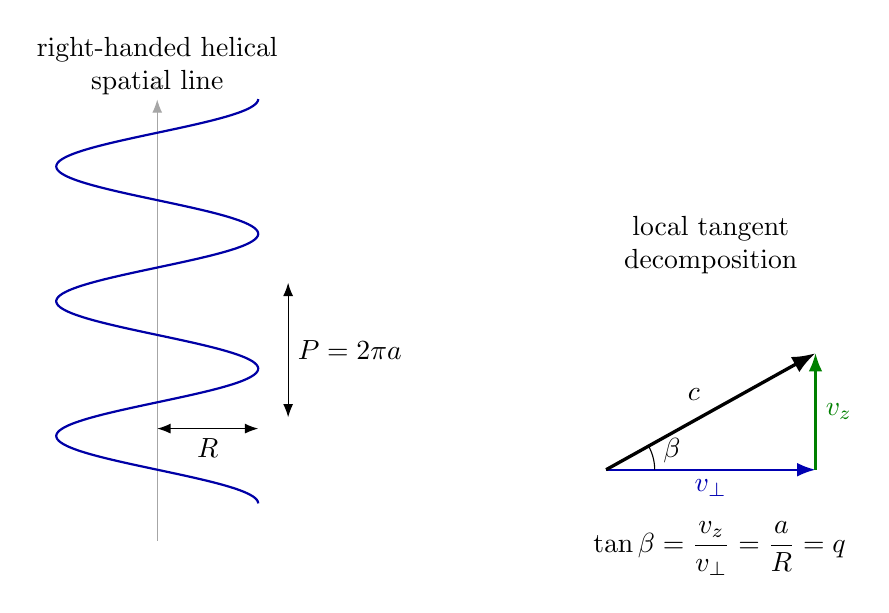
\begin{tikzpicture}[scale=0.95,>=Latex]
  % left: helical side projection
  \begin{scope}[xshift=-3.0cm]
    \draw[->,gray!70] (0,-0.5) -- (0,5.4) node[above] {$z$};
    \draw[blue!65!black,thick,samples=240,domain=0:1080,smooth,variable=\t]
      plot ({1.35*cos(\t)}, {0.005*\t});
    \draw[<->] (0,1.0) -- (1.35,1.0) node[midway,below] {$R$};
    \draw[<->] (1.75,1.15) -- (1.75,2.95) node[midway,right] {$P=2\pi a$};
    \node[align=center] at (0,5.85) {right-handed helical\\spatial line};
  \end{scope}

  % right: tangent decomposition
  \begin{scope}[xshift=3.0cm,yshift=0.45cm]
    \coordinate (O) at (0,0);
    \coordinate (X) at (2.8,0);
    \coordinate (Z) at (2.8,1.558);
    \draw[->,thick,blue!70!black] (O) -- (X) node[midway,below] {$v_\perp$};
    \draw[->,thick,green!50!black] (X) -- (Z) node[midway,right] {$v_z$};
    \draw[->,very thick,black] (O) -- (Z) node[midway,above left] {$c$};
    \draw (0.65,0) arc[start angle=0,end angle=29.09,radius=0.65];
    \node at (0.88,0.25) {$\beta$};
    \node[align=center] at (1.4,3.0) {local tangent\\decomposition};
    \node[align=left,anchor=west] at (-0.3,-1.05) {$\displaystyle \tan\beta=\frac{v_z}{v_\perp}=\frac{a}{R}=q$};
  \end{scope}
\end{tikzpicture}
\caption{Minimal helical spacetime substrate and the geometric meaning of the intrinsic angle $\beta$.  The left panel is a side projection of the helix.  The right panel decomposes local propagation at speed $c$ into transverse and axial components.}
\label{fig:helix}
\end{figure*}

\section{Model postulates and derived helix shape}

The geometry of Sec.~II defines the quantities $R$, $q$, and $\beta$ but does not by itself determine their values.  The present short paper therefore makes three additional assumptions explicit.  They should be read as model postulates to be derived, replaced, or falsified by a future covariant dynamics.

\subsection{Postulate I: gravity--geometry calibration}

Associated with the measured Newton constant is the natural gravitational force/tension scale
\begin{equation}
\tau_G\equiv\frac{c^4}{G}.
\label{eq:tension}
\end{equation}
The first postulate identifies this macroscopic scale with a transverse microscopic scale of the helical substrate,
\begin{equation}
\boxed{\tau_G=\frac{\hbar c}{4R^2}=\frac{hc}{8\pi R^2}}.
\label{eq:calpostulate}
\end{equation}
Equivalently,
\begin{equation}
\boxed{G=\frac{8\pi c^3R^2}{h}}.
\label{eq:Grewrite}
\end{equation}
Equation~\eqref{eq:Grewrite} is used as a calibration relation, not as a prediction of $G$.  Inserting the experimentally measured value of $G$ gives
\begin{equation}
R_G=\sqrt{\frac{hG}{8\pi c^3}}
\simeq8.081275\times10^{-36}\ \mathrm m.
\label{eq:Rvalue}
\end{equation}
Using
\begin{equation}
\ell_{\mathrm P}=\sqrt{\frac{\hbar G}{c^3}},
\label{eq:lp}
\end{equation}
Eq.~\eqref{eq:Rvalue} immediately implies the corollary
\begin{equation}
\boxed{2R_G=\ell_{\mathrm P}}.
\label{eq:Rcal}
\end{equation}
Thus the identification of the Planck length with the helical diameter is not introduced as an additional independent assumption; it follows algebraically from the gravity--geometry calibration postulate.  The measured value used here is the 2022 CODATA recommendation \cite{NISTG},
\begin{equation}
G=6.67430(15)\times10^{-11}\ \mathrm{m^3\,kg^{-1}\,s^{-2}}.
\end{equation}

\subsection{Postulate II: axial rollout energy}

A full helical turn advances axially by
\begin{equation}
P=2\pi a=2\pi qR,
\label{eq:pitchcycle}
\end{equation}
whereas the actual helical path traversed during that turn has length
\begin{equation}
L_{\rm cyc}=2\pi\sqrt{R^2+a^2}
=2\pi R\sqrt{1+q^2}.
\label{eq:Lcycle}
\end{equation}
These two lengths are assigned distinct physical roles.  The axial pitch $P$ measures the \emph{net new spatial extension} generated by one primitive turn, while $L_{\rm cyc}$ measures the \emph{internal propagation path} required to complete that turn.  The second postulate is that the energy cost is proportional to the net axial extension rather than the internal arc length:
\begin{equation}
\boxed{E_{\rm cyc}=\tau_G P
=\frac{c^4}{G}\,2\pi qR.}
\label{eq:Ecycle}
\end{equation}
This axial-versus-arc distinction is structural to the present ansatz.  A future dynamical theory must justify why the conserved or generated quantity couples to $P$ rather than to $L_{\rm cyc}$.

If local propagation along the helical path occurs at $c$, the cycle time is set by the arc length,
\begin{equation}
T_{\rm cyc}=\frac{L_{\rm cyc}}{c}
=\frac{2\pi R\sqrt{1+q^2}}{c}.
\label{eq:Tcycle}
\end{equation}

\subsection{Postulate III: one-cycle phase closure}

Rather than taking $E_{\rm cyc}T_{\rm cyc}=h$ as an isolated quantization rule, we state the third postulate as a phase-closure condition.  A complete primitive turn is required to return the associated quantum phase to itself:
\begin{equation}
\boxed{\Delta\varphi
=\frac{E_{\rm cyc}T_{\rm cyc}}{\hbar}=2\pi.}
\label{eq:phaseclosure}
\end{equation}
Equivalently,
\begin{equation}
E_{\rm cyc}T_{\rm cyc}=h.
\label{eq:actionpostulate}
\end{equation}
This reformulation makes explicit that the appearance of $h$ represents closure of one $2\pi$ phase cycle, not an independently fitted numerical factor.

\subsection{Proposition 1: fixed dimensionless helix shape}

Substituting Eqs.~\eqref{eq:Ecycle} and \eqref{eq:Tcycle} into the phase-closure condition gives
\begin{equation}
4\pi^2\frac{c^3R^2}{G}\,q\sqrt{1+q^2}=h,
\label{eq:dimq}
\end{equation}
or
\begin{equation}
q\sqrt{1+q^2}=X_G,
\qquad
X_G\equiv\frac{hG}{4\pi^2c^3R^2}.
\label{eq:XG}
\end{equation}
Before imposing the gravity calibration explicitly,
\begin{equation}
q(G,h,c;R)=
\sqrt{\frac{\sqrt{1+4X_G^2}-1}{2}}.
\label{eq:qdimensional}
\end{equation}
The associated intrinsic angle can therefore be written directly in terms of the gravitational and quantum constants and the primitive radius:
\begin{equation}
\boxed{
\beta(G,h,c;R)=
\arctan\!\sqrt{
\frac{\sqrt{1+4\left(\dfrac{hG}{4\pi^2c^3R^2}\right)^2}-1}{2}}
}.
\label{eq:betaGconstants}
\end{equation}
Equation~\eqref{eq:betaGconstants} is retained to show explicitly the physical input chain $G\rightarrow R\rightarrow\beta$.  It is not an additional independent prediction because $R$ is itself calibrated from $G$ through Eq.~\eqref{eq:Grewrite}.

Substituting the calibrated value $R=R_G$ causes the dimensional constants to cancel,
\begin{equation}
\boxed{q\sqrt{1+q^2}=\frac{2}{\pi}}.
\label{eq:qeq}
\end{equation}
The positive solution is
\begin{align}
q^2 &= \frac{\sqrt{1+16/\pi^2}-1}{2},\\
q &\simeq 0.5563241800.
\label{eq:qnum}
\end{align}
The cancellation is conceptually important: $G$ fixes the absolute microscopic scale, but once that calibration is imposed, the predicted shape is dimensionless and no longer depends on the numerical magnitude of $G$.

\subsection{Proposition 2: intrinsic geometric angle}

From Eq.~\eqref{eq:betadef},
\begin{align}
\beta_G &= \arctan q \simeq 29.08825^\circ,\\
\boxed{\sin^2\beta_G} &= \boxed{\frac{q^2}{1+q^2}\simeq0.2363477652}.
\label{eq:mainresult}
\end{align}
Up to Eq.~\eqref{eq:mainresult}, no electroweak measurement has entered the construction.

\section{Sensitivity to the transverse calibration}

Because the numerical correspondence discussed below could otherwise be mistaken for a consequence of an arbitrarily chosen Planck-scale radius, it is useful to relax the calibrated relation diagnostically.  Write
\begin{equation}
R=\gamma\ell_{\mathrm P},
\label{eq:gamma}
\end{equation}
without treating $\gamma$ as an additional parameter of the formal model.  Keeping Postulates II and III and the tension scale $\tau_G=c^4/G$, Eq.~\eqref{eq:dimq} becomes
\begin{equation}
q\sqrt{1+q^2}=\frac{1}{2\pi\gamma^2}.
\label{eq:qgamma}
\end{equation}
Thus
\begin{equation}
\sin^2\beta(\gamma)=
\frac{q(\gamma)^2}{1+q(\gamma)^2},
\end{equation}
with $q(\gamma)$ fixed uniquely by Eq.~\eqref{eq:qgamma}.

For orientation, the local sensitivity around the formal calibration is
\begin{equation}
\begin{array}{c|c|c}
\gamma & \beta & \sin^2\beta \\
\hline
0.490 & 29.887^\circ & 0.24829 \\
0.500 & 29.088^\circ & 0.23635 \\
0.50443\;(\gamma_{M_Z}) & 28.741^\circ & 0.23122 \\
0.510 & 28.312^\circ & 0.22493
\end{array}
\label{eq:sensitivityarray}
\end{equation}
where $\gamma_{M_Z}$ denotes the value that would reproduce the PDG $\overline{\mathrm{MS}}$ central value at $M_Z$ under a \emph{direct} identification; it is shown only as a sensitivity diagnostic and is not used in the model.

A percent-level change in the transverse calibration produces a several-percent change in $\sin^2\beta$.  The correspondence is therefore not generic to every radius of order $\ell_{\mathrm P}$.  Conversely, forcing the $M_Z$ central value by direct equality would require $\gamma\simeq0.50443$, only about $0.89\%$ above the formal calibration $\gamma=0.5$.  This proximity is not evidence for a direct identification---renormalization and matching remain unresolved---but it quantifies the sensitivity of the numerical observation.

\section{Covariance and isotropy status}

The right-handed helix in Eq.~\eqref{eq:helix} is introduced as a \emph{local kinematic object}.  The present paper does not assert the existence of a fixed cosmic helix axis embedded in a preferred global Euclidean frame.  Such an interpretation would generically conflict with the observed near-isotropy and Lorentz symmetry of accessible spacetime physics.

A viable completion must therefore do at least one of the following: formulate the helical degree of freedom as an internal or frame/fiber variable; attach local axes relationally to the matter source and recover isotropy under coarse graining; or demonstrate that Lorentz symmetry emerges dynamically from a deeper non-Lorentz microscopic description.  The present ansatz does not choose among these possibilities.  Consequently, no claim of Lorentz covariance is made for Eq.~\eqref{eq:helix} itself.  Recovering a covariant continuum theory without observable preferred-frame effects is a primary consistency requirement for future TEF dynamics.

\section{Empirical numerical correspondence with electroweak weak mixing}

In the Standard Model, the weak mixing angle is not a single scheme-independent observable.  At tree level it is related to the gauge-coupling ratio as in Eq.~\eqref{eq:thetaW}; beyond tree level, on-shell, effective, and $\overline{\mathrm{MS}}$ definitions differ, and the $\overline{\mathrm{MS}}$ quantity runs with the renormalization scale \cite{PDG2026EW}.  Recent precision work has sharpened this point: Erler, Ferro-Hernandez, and Kuberski computed the low-energy $\overline{\mathrm{MS}}$ evolution using lattice-QCD input and perturbation theory \cite{ErlerFerroKuberski2024}, while Spiesberger and Wezorke emphasized the matching conditions required when evolving the weak mixing angle across particle thresholds \cite{SpiesbergerWezorke2024}.  Any eventual TEF--electroweak correspondence must therefore specify a renormalization scheme, a matching scale, and threshold conditions; numerical proximity to a value quoted at one scale is not by itself a valid matching prescription.

The 2026 Particle Data Group review quotes, at the $Z$ scale,
\begin{equation}
\sin^2\widehat\theta_W(M_Z)=0.23122\pm0.00006
\qquad (\overline{\mathrm{MS}}),
\label{eq:pdgmz}
\end{equation}
and an effective leptonic angle near the $Z$ pole of
\begin{equation}
\sin^2\theta_{\rm eff}^{\ell}=0.23154\pm0.00006.
\end{equation}
For context, the same review discusses low-energy determinations such as
\begin{equation}
\sin^2\widehat\theta_W(161\,\mathrm{MeV})=0.2403\pm0.0013
\end{equation}
from SLAC E158, and an atomic-parity-violation interpretation
\begin{equation}
\sin^2\widehat\theta_W(2.4\,\mathrm{MeV})=0.2349\pm0.0018,
\end{equation}
illustrating the scale and scheme dependence \cite{PDG2026EW}.

The TEF geometric value is
\begin{equation}
\sin^2\beta=0.2363478.
\end{equation}
Relative to the $\overline{\mathrm{MS}}$ value at $M_Z$, the difference is
\begin{equation}
\Delta=0.00513,
\qquad
\frac{\Delta}{\sin^2\widehat\theta_W(M_Z)}\simeq2.22\%.
\end{equation}
This difference is far larger than the quoted experimental/theoretical uncertainty at the $Z$ scale.  Therefore Eq.~\eqref{eq:mainresult} cannot presently be identified directly with Eq.~\eqref{eq:pdgmz}.

Nevertheless, the numerical proximity is nontrivial in the restricted sense relevant here: a dimensionless number produced by a gravity-calibrated microscopic geometry, without electroweak input, falls in the same $\sim0.23$--$0.24$ regime as the running weak-mixing parameter.  This motivates a stronger but still explicitly conjectural interpretation: the intrinsic TEF helix angle may represent a primitive geometric reference angle underlying electroweak mixing,
\begin{equation}
\boxed{\theta_{W,\mathrm{geom}}^{\TEF}\stackrel{?}{=}\beta_G},
\qquad
q=\tan\beta_G \stackrel{?}{\longleftrightarrow} \frac{g'}{g}.
\label{eq:candidate}
\end{equation}
Under this interpretation, measured quantities conventionally denoted by $\theta_W$ would be scale-, scheme-, and environment-dependent effective realizations rather than the primitive geometric angle itself.  This is a candidate geometric explanation of the origin of the weak mixing angle, not yet a derivation: a field-theoretic matching or renormalization prescription must still connect $\beta_G$ to the conventional $\theta_W(\mu)$.

\begin{table*}[t]
\caption{Numerical comparison.  The TEF value is not fitted to any electroweak datum.  Standard-Model entries are scheme- and scale-dependent and should not be treated as measurements of one universal constant.}
\label{tab:compare}
\centering
\begin{ruledtabular}
\begin{tabular}{lcc}
Quantity & Value & Comment \\
\hline
$\sin^2\beta$ & $0.2363478$ & TEF geometric output \\
$\sin^2\widehat\theta_W(M_Z)$ & $0.23122\pm0.00006$ & PDG 2026, $\overline{\mathrm{MS}}$ \\
$\sin^2\theta_{\rm eff}^{\ell}$ & $0.23154\pm0.00006$ & PDG 2026, $Z$ pole \\
$\sin^2\widehat\theta_W(161\,\mathrm{MeV})$ & $0.2403\pm0.0013$ & SLAC E158 interpretation \\
$\sin^2\widehat\theta_W(2.4\,\mathrm{MeV})$ & $0.2349\pm0.0018$ & atomic parity violation \\
\end{tabular}
\end{ruledtabular}
\end{table*}

\section{Interpretation, novelty boundary, and falsifiability}

The construction separates inspiration from inference.  Euler's formula motivates the representation of transverse rotation by a phase variable, but no electroweak conclusion follows from Euler's identity alone.  The physical content begins only after TEF postulates that generated spatial extension has the helical geometry of Eq.~\eqref{eq:helix} and assigns dynamical meaning to its axial rollout.

The important distinction in this construction is between scale and shape.  Postulate I calibrates the dimensional parameter $R$ from the gravitational sector, while Postulates II and III determine a dimensionless shape $q$ and therefore an intrinsic angle $\beta$.  The Planck-diameter relation $2R=\ell_{\mathrm P}$ is a corollary of that calibration rather than an additional independent input.  The candidate electroweak connection concerns the shape, not the absolute length.

A geometric interpretation of the weak mixing angle is not new.  Noncommutative-geometric approaches relate Standard-Model gauge couplings to deeper geometric data \cite{Connes2006,ChamseddineConnesMarcolli2006}, and the recent colored-gravity construction of Ref.~\cite{Monjo2025} is particularly close in motivation because it seeks a gravitational/geometric origin for $\theta_W$.  The mechanisms are nevertheless distinct.  In Ref.~\cite{Monjo2025}, weak-mixing values arise from the generator and representation structure of a $U(1,3)$ gauge-gravity theory.  Here, by contrast, $q=a/R$ is the pitch-to-radius ratio of a local helical spacetime substrate, and $\sin^2\beta$ is the squared axial fraction of the local rollout velocity.  To our knowledge from a targeted but necessarily non-exhaustive literature search, the specific identification $a/R=\tan\beta$ as a candidate weak-mixing geometry together with the constraint in Eq.~\eqref{eq:qeq} has not been previously formulated.  This is a limited priority statement about the present ansatz, not a claim of priority for geometric explanations of electroweak mixing in general.

\subsection{Why the numerical correspondence is worth testing}

The numerical comparison should be interpreted with two constraints in mind.  First, the construction is not parameter free: Eq.~\eqref{eq:calpostulate} fixes the absolute transverse scale by a gravitational calibration, while Eqs.~\eqref{eq:Ecycle} and \eqref{eq:phaseclosure} are structural and quantization postulates.  The result is therefore not a first-principles Standard-Model prediction.  Second, however, the electroweak number is not used as a fitting target anywhere in the chain
\begin{equation}
G_{\rm exp}\;\longrightarrow\;R_G\;\longrightarrow\;q\;\longrightarrow\;\beta_G.
\label{eq:inferencechain}
\end{equation}
Once the stated assumptions are fixed, the value in Eq.~\eqref{eq:mainresult} is no longer adjustable.  The interest of the result lies specifically in this separation of sectors: a scale calibrated from gravity participates in a geometric construction whose dimensionless output lands in the numerical regime of electroweak mixing.

This type of cross-sector coincidence is weaker than a derivation but stronger than a post-hoc fit only to the extent that the assumptions are independently motivated and kept fixed.  The appropriate next test is therefore not to choose a renormalization scale at which the Standard-Model curve happens to pass closest to Eq.~\eqref{eq:mainresult}.  Rather, a viable continuation must derive a matching relation between the helical degree of freedom and electroweak gauge fields, after which the standard running and threshold machinery \cite{ErlerFerroKuberski2024,SpiesbergerWezorke2024} can be applied without introducing a new free angle.  Failure to obtain such a map would leave the present numerical correspondence as an unexplained coincidence.

The present ansatz remains incomplete in several decisive ways:
\begin{enumerate}[leftmargin=*,label=(\roman*)]
\item The helical substrate has not yet been derived from a covariant action or microscopic dynamical theory.
\item The gravity--geometry calibration in Eq.~\eqref{eq:calpostulate} has not yet been derived from a covariant action.
\item The identification of cycle energy with the gravitational line tension times the \emph{axial} generated length, rather than the helical arc length, is a structural postulate that requires deeper justification.
\item The phase-closure condition in Eq.~\eqref{eq:phaseclosure} is a quantization postulate, not yet a theorem of the framework.
\item No derivation has yet shown that the helical degrees of freedom generate the gauge group $SU(2)_L\times U(1)_Y$ or that $q$ must equal $g'/g$.
\item A quantitative renormalization-group or matching calculation is required.  If no consistent mapping carries a geometric boundary value associated with Eq.~\eqref{eq:mainresult} into observed weak-mixing data, the electroweak correspondence fails even if the numerical proximity remains.
\item A microscopic right-handed structure must be reconciled with the observed near-isotropy and Lorentz symmetry of macroscopic spacetime.  A viable TEF theory must explain why no unacceptable preferred-frame or anisotropy signal survives at accessible scales.
\end{enumerate}

These limitations are useful only insofar as they make the proposal testable and falsifiable.  The numerical observation in Eq.~\eqref{eq:mainresult} is not offered as proof of TEF; rather, it identifies a concrete target for a future dynamical theory.

\section{Conclusion}

We have examined a minimal helical model of generated spatial extension motivated by TEF.  Inspired by Euler's representation of planar rotation through complex phase, the helix couples transverse phase rotation to axial rollout through a common parameter.  The construction separates a dimensional primitive radius $R$ from a dimensionless helix shape $q=a/R$.  Measured gravity is used openly to calibrate $R$ through the postulated relation $G=8\pi c^3R^2/h$, which gives $R_G=\sqrt{hG/(8\pi c^3)}=\ell_{\mathrm P}/2$; TEF does not claim to predict $G$ in this paper.  Assigning the net axial rollout length the gravitational line-tension energy cost $c^4/G$ while using the helical arc length to set the propagation time, and imposing one-cycle phase closure, then gives
\begin{equation}
q\sqrt{1+q^2}=\frac{2}{\pi}
\end{equation}
and therefore
\begin{equation}
\sin^2\beta\simeq0.236348.
\end{equation}
The intrinsic TEF angle $\beta$ is geometrically well defined: $\sin^2\beta=v_z^2/c^2$ is the normalized squared axial component of the local helical rollout.

We therefore propose $\beta_G\simeq29.088^\circ$ as a candidate primitive geometric reference angle that may underlie weak mixing.  The resulting number is numerically close to, but not equal to, conventional weak-mixing parameters.  In particular, it differs by about $2.22\%$ from the 2026 PDG $\overline{\mathrm{MS}}$ value at $M_Z$, so a direct identification is excluded at present.  What makes the coincidence potentially informative is the separation of inputs: no electroweak observable is used to obtain the TEF value.  A successful continuation of the program would need to derive, rather than assume, a field-theoretic map between the helical geometry and electroweak gauge couplings and to reproduce their scale dependence.  The sensitivity analysis also shows that the correspondence is not produced by an arbitrary order-Planck radius: small changes in the transverse calibration move the geometric angle appreciably, making the calibration itself part of what a deeper theory must justify.

The broader literature supplies two useful benchmarks for what must come next.  Modern calculations of the running weak angle make the required field-theoretic matching quantitatively precise \cite{ErlerFerroKuberski2024,SpiesbergerWezorke2024}, while current emergent-spacetime programs demonstrate that recovering continuum dynamics from microscopic degrees of freedom is a concrete technical problem rather than only an ontological statement \cite{CalcinariDelhomOriti2026,DekhilGrecoLiberatiOriti2026,Rainer2026}.  TEF will become competitive with such programs only if the present kinematic ansatz can be embedded in a dynamical and covariant framework.

Thus the present result should be regarded as a sharply stated geometric clue rather than a completed unification: a gravity-calibrated spacetime ansatz produces an intrinsic dimensionless angle in the electroweak numerical regime.  It is precisely this quantitative outcome, rather than the novelty of the ansatz itself, that motivates further investigation of the underlying emergent-spacetime hypothesis.

\begin{acknowledgments}
The author thanks the broader community of researchers whose work on geometric formulations of gauge theory and precision electroweak physics provides the context in which this exploratory ansatz can be tested.
\end{acknowledgments}

\begin{thebibliography}{99}

\bibitem{PDG2026EW}
S. Navas \textit{et al.} (Particle Data Group),
``Electroweak Model and Constraints on New Physics,''
\textit{Review of Particle Physics} (2026),
\url{https://pdg.lbl.gov/2026/reviews/rpp2026-rev-standard-model.pdf}.

\bibitem{NISTG}
E. Tiesinga, P. J. Mohr, D. B. Newell, and B. N. Taylor,
``CODATA Recommended Values of the Fundamental Physical Constants: 2022,''
National Institute of Standards and Technology (2024 update),
\url{https://physics.nist.gov/cgi-bin/cuu/Value?bg=}.

\bibitem{Connes2006}
A. Connes,
``Noncommutative Geometry and the Standard Model with Neutrino Mixing,''
arXiv:hep-th/0608226 (2006),
\url{https://arxiv.org/abs/hep-th/0608226}.

\bibitem{ChamseddineConnesMarcolli2006}
A. H. Chamseddine, A. Connes, and M. Marcolli,
``Gravity and the Standard Model with Neutrino Mixing,''
arXiv:hep-th/0610241 (2006),
\url{https://arxiv.org/abs/hep-th/0610241}.

\bibitem{Monjo2025}
R. Monjo,
``Weak mixing angle under $U(1,3)$ colored gravity,''
arXiv:2502.11236 [hep-ph, gr-qc, hep-th] (2025),
\url{https://arxiv.org/abs/2502.11236}.

\bibitem{LiuLowYin2025}
Q. Liu, I. Low, and Z. Yin,
``A Quantum Computational Determination of the Weak Mixing Angle in the Standard Model,''
arXiv:2509.18251 [hep-ph] (2025),
\url{https://arxiv.org/abs/2509.18251}.

\bibitem{ErlerFerroKuberski2024}
J. Erler, R. Ferro-Hernandez, and S. Kuberski,
``Theory Driven Evolution of the Weak Mixing Angle,''
arXiv:2406.16691 [hep-ph] (2024),
\url{https://arxiv.org/abs/2406.16691}.

\bibitem{SpiesbergerWezorke2024}
H. Spiesberger and S. Wezorke,
``Matching the Weak Mixing Angle at Low Energies,''
arXiv:2406.17889 [hep-ph] (2024),
\url{https://arxiv.org/abs/2406.17889}.

\bibitem{Rainer2026}
M. Rainer,
``Gravitation and Spacetime: Emergent from Spinor Interactions -- How?,''
arXiv:2601.00070 [gr-qc] (2026),
\url{https://arxiv.org/abs/2601.00070}.

\bibitem{CalcinariDelhomOriti2026}
A. Calcinari, A. Delhom, and D. Oriti,
``Collective excitations in quantum gravity condensates,''
arXiv:2605.18977 [gr-qc] (2026),
\url{https://arxiv.org/abs/2605.18977}.

\bibitem{DekhilGrecoLiberatiOriti2026}
R. Dekhil, F. Greco, S. Liberati, and D. Oriti,
``Emergent scalar field dynamics in a cosmological spacetime from GFT quantum gravity,''
arXiv:2608.12003 [gr-qc] (2026),
\url{https://arxiv.org/abs/2608.12003}.

\end{thebibliography}

\end{document}
